
The given equation can be expressed as
\begin{align}
\vec{x}^T \myvec{3 & 0\\0 & 0}\vec{x}+ 2\myvec{-1 \\ \frac{-1}{2}}\vec{x}+\frac{1}{3}=0
\end{align}
with
\begin{align}
\vec{V} = \myvec{3 & 0 \\ 0 & 0},\vec{u}=\myvec{-1 \\ \frac{-1}{2}},f=\frac{1}{3}
\end{align}
Using eigenvalue decomposition,
\begin{align}
\vec{D} = \myvec{0 & 0\\0 & 3} ,\vec{P}=\myvec{0 & 1\\1 & 0}
\end{align}
Thus,
\begin{align}
\myvec{\vec{u}^T + \eta\vec{p_1}^T \\ \vec{V}}\vec{c} &= \myvec{-f \\ \eta\vec{p_1}-\vec{u}} 
\\
\implies \myvec{-1 & -1 \\ 3 & 0 \\ 0 & 0}\vec{c} &= \myvec{\frac{-1}{3}\\ 1 \\ 0} \\
\implies  \myvec{-1 & -1 \\ 3 & 0}\vec{c} &= \myvec{\frac{-1}{3}\\ 1}
\\
\implies \vec{c} &= \myvec{\frac{1}{3}\\0}
\end{align}
$\because$
\begin{align}
\vec{p_1}^T\vec{c} &= \myvec{0 & 1}\myvec{\frac{1}{3}\\0}
\\
&= 0
\\
\vec{p_2}^T\vec{V}\vec{p_2} &= \myvec{1 & 0}\myvec{3 & 0\\0& 0}\myvec{1 \\ 0}
\\
&= 3,
\end{align}
$\because$
\begin{align}
(\vec{p_1}^T\vec{c})(\vec{p_2}^T\vec{V}\vec{p_2}) = 0
\end{align}
Thus, the given equation has  real and equal roots which can be verified from Fig. \ref{quadforms/2/25/Roots of}.  
%
\begin{figure}[!ht]
\centering
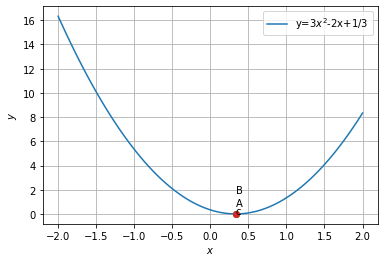
\includegraphics[width=\columnwidth]{solutions/su2021/2/25/download (3).png}
\caption{Roots of $3x^2 -2x + 1/3 = 0$ }
\label{quadforms/2/25/Roots of}
\end{figure}




